\documentclass[12pt]{article}
\usepackage{amsmath,amssymb,amsfonts}
\usepackage{graphicx}
% Pages Settings

%\usepackage[margin = 1in]{geometry}
\usepackage[top = 1in,bottom =1in,left = 0.5in, right = 0.5in]{geometry}
%\usepackage[top = 1in,bottom =1in,left = 0.5in, right = 0.5in,paperwidth=5in,paperheight=7in]{geometry}
%\usepackage[letterpaper]{geometry}


% Using Macros
\def\My_Eq{y = x^2+1}


\begin{document}
	\begin{figure}
	\centering
	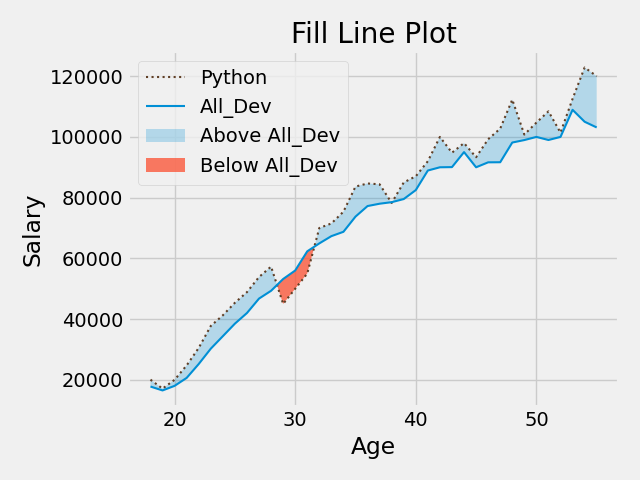
\includegraphics[scale=0.75]{Fill_Py}
	\caption{Fill Line Plot}
	\end{figure}
	\begin{enumerate}
	\item This is from My Macro : $\left[\My_Eq\right]$ 
	\item This is a Trigonometric Equation $ y = sin\theta $
	\item This is a Log Function $ f(x) = log_{10} X$
	\item The Mathematical Notation of the set of all Real Numbers is $ \mathbb{R} $.
	\item The Mathematical Notation of the set of all Integer Numbers is $ \mathbb{Z} $.
	\item The Mathematical Notation of the set of all Rational Numbers is $ \mathbb{Q} $.
	\item This is a Differntial Fraction: $\left(  \dfrac{\sqrt[4]{x^2+4}}{\left.  \dfrac{dy}{dx} \right|x=10}  \right)$ 
	\end{enumerate}
\end{document}